\chapter[Hierarchical Selective Classification]{Hierarchical Selective Classification of European Land Use / Land Cover using pixel-based uncertainty}
\label{cha:chapter4}
\vspace*{\fill}
This chapter is based on:
\\
\\
% Full citation of the published (or submitted/in review) article
% This refers to the article key in the refs.bib file.
\fullcite{witjes2024hierarchical}
\newpage

\section*{Abstract}
HAS TO HAVE ALL SECTIONS

CAN BE SHORT AND UNCOOKED

SOME CLEAR RESULTS
\newpage

\section{Introduction}
Land cover is important. 

\subsection{Where do you get data?}

It is important to have independent training and validation samples. The best open validation samples for Europe are the LUCAS points \citep{dandrimont2021lucas,dandrimont2020harmonised} because of their sound sampling design, large legend, and covering multiple years \citep{venter2022global}

Corine is super cool and can be harvested for training data\citep{witjes2022spatiotemporal,witjes2024iterative}
but doesn't have all classes for LUCAS validation \citep{dandrimont2021lucas} if you want to go beyond high level classes or throw a lot away \citep{pflugmacher2019mapping}.
Eurocrops is super cool and provides a lot of classes missing in CORINE \citep{schneider2023eurocrops}
OpenStreetMap is super cool and can be used to supplement training datasets with additional classes [SOURCE NEEDED] and can also be used to filter spurious labels extracted from CORINE \citep{witjes2022spatiotemporal}



\section{Methods}

\begin{figure}[H]
    \centering
    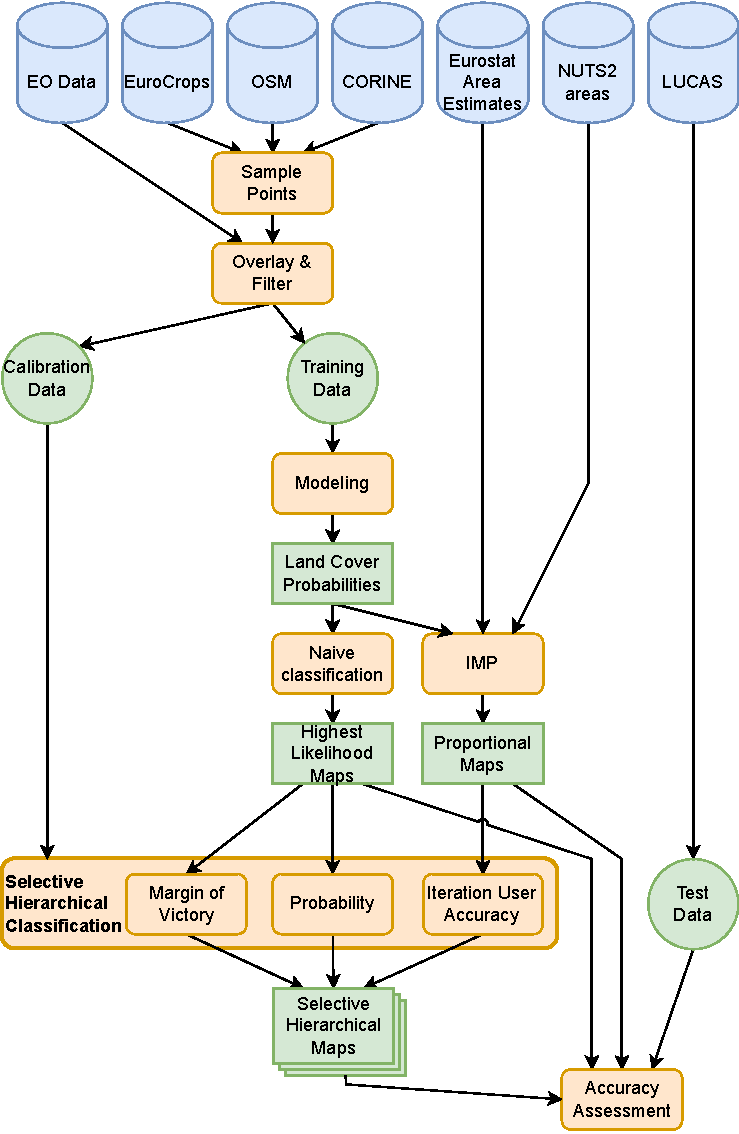
\includegraphics[width=\textwidth]{figs_05/fig_methodology.pdf}
    \caption{Caption}
    \label{fig:05_methodology}
\end{figure}

\subsection{Selection of study area}

We obtained Nomenclature of Territorial Units for Statistics (NUTS) administrative boundaries from EuroStat. %https://ec.europa.eu/eurostat/web/gisco/geodata/reference-data/administrative-units-statistical-units/nuts
We matched level 2 NUTS areas to the earliest LUCAS survey since each update (See Table~\ref{tab:05_NUTS_LUCAS}). 

We selected all NUTS2 areas:
1. For which LUCAS land cover area estimates were available;
2. For which more than 500 LUCAS points were available;
2. Whose area was below the largest 1\% surface area among NUTS2 areas (to maintain computational feasibility)

We randomly selected up to four NUTS2 area/year combinations each country.

\begin{table}[H]
    \centering
    \begin{tabular}{c|c}
         NUTS update year &  LUCAS survey year\\
         2006 & 2006 \\
         2010 & 2012 \\
         2013 & 2015 \\
         2016 & 2018 \\
    \end{tabular}
    \caption{Caption}
    \label{tab:05_NUTS_LUCAS}
\end{table}

\subsection{Legend harmonization}
% https://docs.google.com/spreadsheets/d/1UJrbdGJgrXlW_WnSoDVIhf68dz8XoiWrZW6WVeR5lPw/edit#gid=1654270911
For some classes, either no area estimates or no training data was found. This required us to merge some classes, and aggregate others to a higher level in the hierarchical legend. Table \ref{tab:05_legend_harmonization} shows which LUCAS classes were aggregated and merged, and for what reason.

% Please add the following required packages to your document preamble:
% \usepackage{multirow}
\begin{table}[]
\label{tab:05_legend_harmonization}
% https://docs.google.com/spreadsheets/d/1UJrbdGJgrXlW_WnSoDVIhf68dz8XoiWrZW6WVeR5lPw/edit#gid=213241018
\begin{tabular}{l{2cm}lll}
LUCAS land cover class                        & Training data source    & Used land cover class                                 & Reason for aggregation/omission                           \\
A11: Buildings with one to three floors       & \multirow{2}{*}{corine} & \multirow{2}{*}{A10: Roofed built-up areas}           & No training data                                          \\
A12: Buildings with more than three floors    &                         &                                                       & No training data                                          \\
\multirow{2}{*}{A13: Greenhouses}             & openstreetmap           & \multirow{2}{*}{A13: Greenhouses}                     &                                                           \\
                                              & eurocrops               &                                                       &                                                           \\
A21: Non built-up area features               & \multirow{2}{*}{corine} & \multirow{2}{*}{A20: Artificial non-built up areas}   & No training data                                          \\
A22: Non built-up linear features             &                         &                                                       & No training data                                          \\
B11: Common wheat                             & eurocrops               & B11: Common wheat                                     &                                                           \\
B12: Durum wheat                              & eurocrops               & B12: Durum wheat                                      &                                                           \\
B13: Barley                                   & eurocrops               & B13: Barley                                           &                                                           \\
B14: Rye                                      & eurocrops               & B14: Rye                                              &                                                           \\
B15: Oats                                     & eurocrops               & B15: Oats                                             &                                                           \\
B16: Maize                                    & eurocrops               & B16: Maize                                            &                                                           \\
B17: Rice                                     & corine                  & B17: Rice                                             &                                                           \\
B17: Rice                                     & eurocrops               & B17: Rice                                             &                                                           \\
B18: Triticale                                & eurocrops               & B18: Triticale                                        &                                                           \\
B19: Other cereals                            & eurocrops               & \multirow{2}{*}{B19: Other cereals}                   &                                                           \\
B54: Mixed cereals for fodder                 &                         &                                                       & No training data                                          \\
B21: Potatoes                                 & eurocrops               & B21: Potatoes                                         &                                                           \\
B22: Sugar beet                               & eurocrops               & B22: Sugar beet                                       &                                                           \\
B23: Other root crops                         & eurocrops               & B23: Other root crops                                 &                                                           \\
B31: Sunflower                                & eurocrops               & B31: Sunflower                                        &                                                           \\
B32: Rape and turnip rape                     & eurocrops               & B32: Rape and turnip rape                             &                                                           \\
B33: Soya                                     & eurocrops               & B33: Soya                                             &                                                           \\
B34: Cotton                                   & eurocrops               & \multirow{2}{*}{B35: Other fibre and olaginous crops} & No training data in eurocrops, despite presence in legend \\
B35: Other fibre and olaginous crops          & eurocrops               &                                                       &                                                           \\
B36: Tobacco                                  & eurocrops               & B36: Tobacco                                          &                                                           \\
B37: Other non-permanent industrial crops     & eurocrops               & B37: Other non-permanent industrial crops             &                                                           \\
B41: Dry pulses                               & eurocrops               & B41: Dry pulses                                       &                                                           \\
B42: Tomatoes                                 & eurocrops               & B42: Tomatoes                                         &                                                           \\
B43: Other fresh vegetables                   & eurocrops               & B43: Other fresh vegetables                           &                                                           \\
B44: Floriculture and ornamental plants       & eurocrops               & B44: Floriculture and ornamental plants               &                                                           \\
B45: Strawberries                             & eurocrops               & B45: Strawberries                                     &                                                           \\
B51: Clovers                                  & eurocrops               & B51: Clovers                                          &                                                           \\
B52: Lucerne                                  & eurocrops               & B52: Lucerne                                          &                                                           \\
B53: Other leguminous and mixtures for fodder & eurocrops               & B53: Other leguminous and mixtures for fodder         &                                                           \\
B55: Temporary grasslands                     & eurocrops               & B55: Temporary grasslands                             &                                                           \\
B71: Apple fruit                              & eurocrops               & B71: Apple fruit                                      &                                                           \\
B72: Pear fruit                               & eurocrops               & B72: Pear fruit                                       &                                                           \\
B73: Cherry fruit                             & eurocrops               & B73: Cherry fruit                                     &                                                           \\
B74: Nuts trees                               & eurocrops               & B74: Nuts trees                                       &                                                           \\
B75: Other fruit trees and berries            & eurocrops               & B75: Other fruit trees and berries                    &                                                           \\
B76: Oranges                                  &                         & \multirow{2}{*}{B77: Other citrus fruit}              & No training data                                          \\
B77: Other citrus fruit                       & eurocrops               &                                                       &                                                           \\
\multirow{2}{*}{B81: Olive groves}            & corine                  & \multirow{2}{*}{B81: Olive groves}                    &                                                           \\
                                              & eurocrops               &                                                       &                                                           \\
\multirow{2}{*}{B82: Vineyards}               & corine                  & \multirow{2}{*}{B82: Vineyards}                       &                                                           \\
                                              & eurocrops               &                                                       &                                                           \\
B83: Nurseries                                & eurocrops               & B83: Nurseries                                        &                                                           \\
B84: Permanent industrial crops               & eurocrops               & B84: Permanent industrial crops                       &                                                           \\
C10: Broadleaved woodland                     & corine                  & C10: Broadleaved woodland                             &                                                           \\
C21: Spruce dominated coniferous woodland     & \multirow{3}{*}{corine} & \multirow{3}{*}{C20: Coniferous woodland}             & No area estimates                                         \\
C22: Pine dominated coniferous woodland       &                         &                                                       & No area estimates                                         \\
C23: Other coniferous woodland                &                         &                                                       & No area estimates                                         \\
C31: Spruce dominated mixed woodland          & \multirow{3}{*}{corine} & \multirow{3}{*}{C30: Mixed woodland}                  & No area estimates                                         \\
C32: Pine dominated mixed woodland            &                         &                                                       & No area estimates                                         \\
C33: Other mixed woodland                     &                         &                                                       & No area estimates                                         \\
D10: Shrubland with sparse tree cover         & corine                  & D10: Shrubland with sparse tree cover                 &                                                           \\
D20: Shrubland without tree cover             & corine                  & D20: Shrubland without tree cover                     &                                                           \\
E10: Grassland with sparse tree/shrub cover   &                         & \multirow{4}{*}{E00: Grassland}                       & No training data                                          \\
E20: Grassland without tree/shrub cover       & eurocrops               &                                                       & No area estimates                                         \\
E20: Grassland without tree/shrub cover       & corine                  &                                                       & No area estimates                                         \\
E30: Spontaneously re-vegetated surfaces      &                         &                                                       & no training data                                          \\
F10: Rocks and stones                         & \multirow{3}{*}{corine} & \multirow{3}{*}{F00: Bare land and lichens/moss}      & No area estimates                                         \\
F20: Sand                                     &                         &                                                       & No area estimates                                         \\
F40: Other bare soil                          &                         &                                                       & No area estimates                                         \\
G11: Inland fresh water bodies                & \multirow{8}{*}{corine} & \multirow{8}{*}{G00: Water areas}                     & No area estimates                                         \\
G12: Inland salty water bodies                &                         &                                                       & No area estimates                                         \\
G21: Inland fresh running water               &                         &                                                       & No area estimates                                         \\
G22: Inland salty running water               &                         &                                                       & No area estimates                                         \\
G30: Transitional water bodies                &                         &                                                       & No area estimates                                         \\
G30: Transitional water bodies                &                         &                                                       & No area estimates                                         \\
G40: Sea and ocean                            &                         &                                                       & No area estimates                                         \\
G50: Glaciers, permanent snow                 &                         &                                                       & No area estimates                                         \\
H11: Inland marshes                           & \multirow{5}{*}{corine} & H11: Inland marshes                                   &                                                           \\
H12: Peatbogs                                 &                         & H12: Peatbogs                                         &                                                           \\
H21: Salt marshes                             &                         & H21: Salt marshes                                     &                                                           \\
H22: Salines and other chemical deposits      &                         & H22: Salines and other chemical deposits              &                                                           \\
H23: Intertidal flats                         &                         & H23: Intertidal flats                                 &                                                          
\end{tabular}
\end{table}

\subsection{Training Data}
We extracted polygons from CORINE, EuroCrops and OpenStreetmap. Table~\ref{tab:05_sources} shows the training data source per LUCAS class.

We randomly sampled points from polygons. One point minimum, one extra point per X square meters of polygon surface, to a maximum of X points per polygon.

We filtered the training data with Copernicus HRL layers and OpenStreetmap building and roads data. 

\subsection{Validation Data}

\section{Results}
\subsection{Training data}



\subsection{Validation data}

Sampling up to four NUTS2 area/year combinations with more than 500 LUCAS points and available area estimates resulted in 93 selected areas. Figure~\ref{fig:05_lucas_aoi} shows the selected areas and gives an overview of the level 1 land cover classes of the LUCAS points they contain. Figure~\ref{fig:05_lucas_aoi_counts} shows the number of validation points per class across all areas.

\begin{figure}[h]
    \centering
    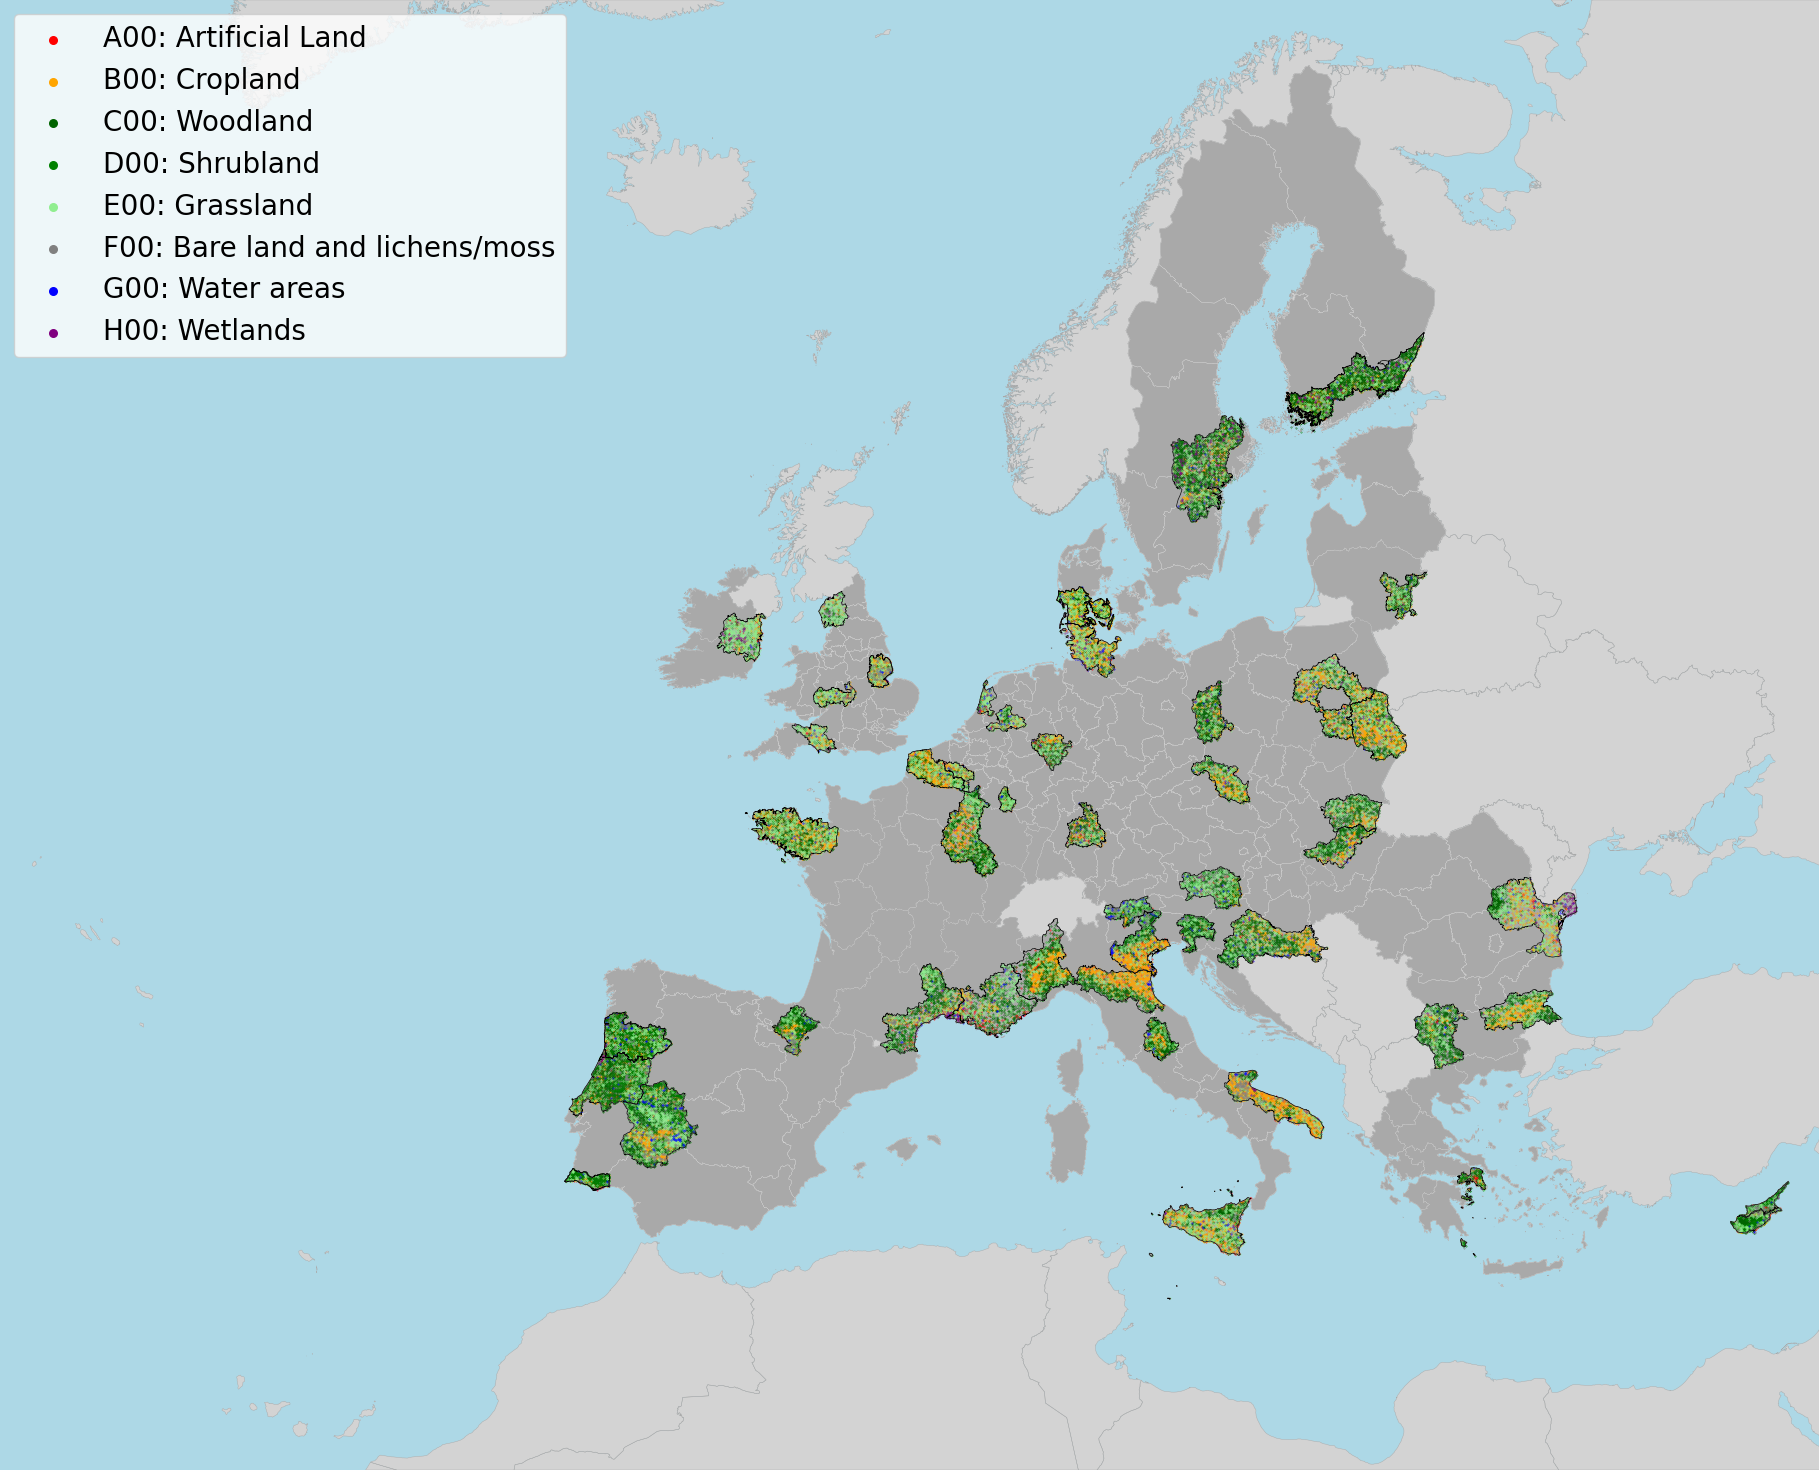
\includegraphics[width=\textwidth]{figs_05/fig_lucas_aoi.png}
    \caption{LUCAS points in sampled NUTS2 areas, used for validation of all land cover maps}
    \label{fig:05_lucas_aoi}
\end{figure}

\begin{figure}[h]
    \centering
    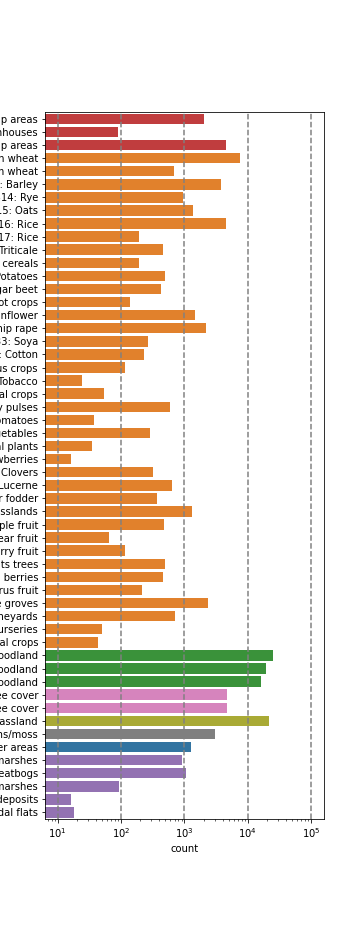
\includegraphics[width=\textwidth]{figs_05/fig_lucas_aoi_counts.png}
    \caption{Number of LUCAS points per LUCAS class used to validate the land cover maps, colored based on their level 1 class.}
    \label{fig:05_lucas_aoi_counts}
\end{figure}

\section{Discussion}

    \subsection{Legend}
        We lost a lot of detail in our legend because we needed 1) training data, 2) area estimates, and 3) validation points. We had training data for a lot of water \& bare land subclasses. It would be good if Eurostat made area estimates for all LUCAS land cover classes; we could have included them.